\documentclass[main.tex]{subfiles} % Subfile-Class

%==============================================================================%
%                                   Subfile                                    %
%==============================================================================%

\begin{document}

% Template

\section{Funktionsbeschreibung}

\subsection{Übersicht}

Im Rahmen dieses Projekts wurde ein autonomes Fahrzeug entwickelt, das sich selbstständig 
durch ein Wegenetzwerk navigieren kann. Das System wurde speziell dafür konzipiert, dynamisch 
auf Hindernisse und Einschränkungen zu reagieren und stets den optimalen Weg von einem 
definierten Startpunkt zu einem Zielpunkt zu finden.

\begin{figure}[H]
    \centering
    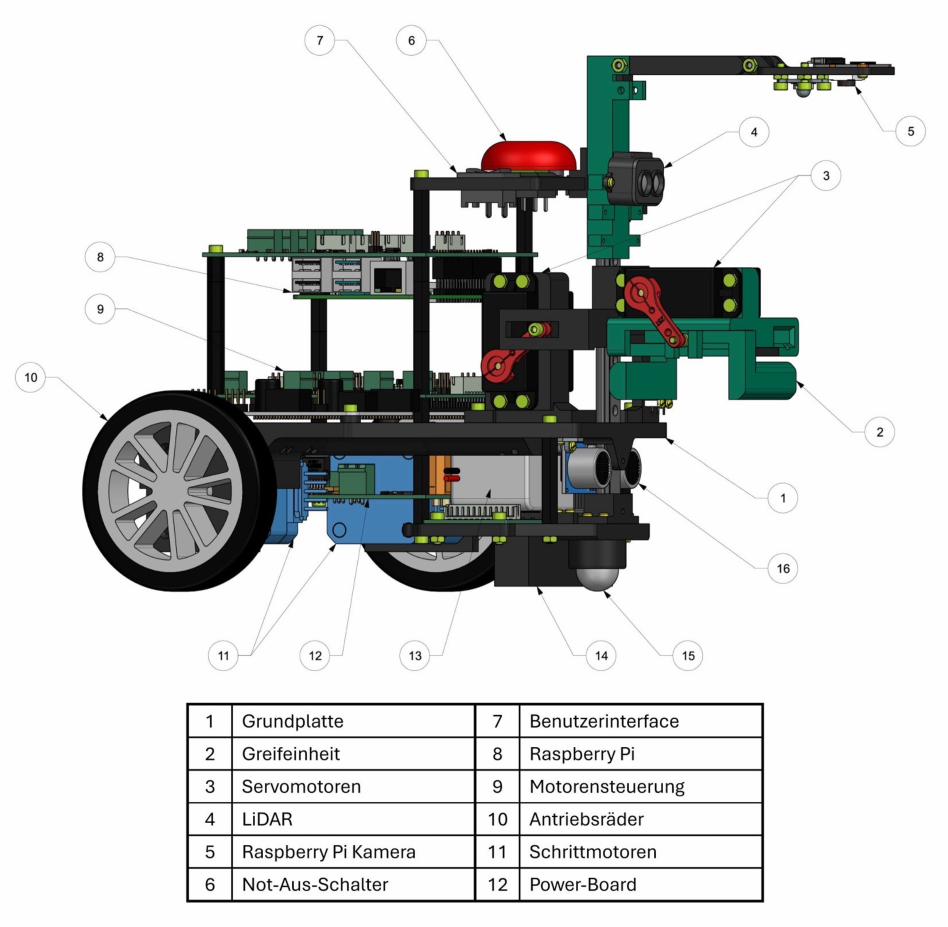
\includegraphics[width = 1.0\linewidth]{./Figures/Gesamtuebersicht-Fahrzeug.pdf}
    \caption{Gesamtübersicht des Fahrzeugs mit Bildlegende}~\label{fig:Gesamtuebersicht}
\end{figure}

Das Fahrzeug zeichnet sich durch eine modulare Bauweise aus, welche die Integration verschiedenster 
Technologien ermöglicht. Die zentralen Komponenten sind:

\paragraph{Chassis und Antrieb}

Das Fahrzeug besitzt ein dreirädriges Chassis mit zwei angetriebenen Rädern und einem 
stabilisierenden Auflagepunkt. Die Bewegung erfolgt über präzise steuerbare Schrittmotoren, 
die eine hohe Wendigkeit ermöglichen. Das Chassis ist leicht und stabil genug, um den 
Gewichtsvorgaben zu entsprechen.

\paragraph{Sensorik}

Zur Umgebungswahrnehmung kommen verschiedene Sensoren zum Einsatz:

\begin{itemize}
  \item \textbf{Liniensensoren}: Erfassen die UV-aktive Leitlinie und erkennen Knotenpunkte.
  \item \textbf{Ultraschallsensoren}: Detektieren Hindernisse im Nahbereich.
  \item \textbf{LiDAR}: Identifiziert auf definierter Höhe Pylonen, welche gesperrte Wegpunkte markieren.
  \item \textbf{Kamera}: Erkennt Knotenpunkte frühzeitig und identifiziert das Ziel eindeutig.
\end{itemize}

Alle Sensoren liefern gemeinsam ein Echtzeitbild der Umgebung und bilden die Grundlage für Navigation und Reaktion.


\paragraph{Steuerungseinheit}

Ein Mikrocontroller-System verarbeitet die Sensordaten, steuert die Motoren und führt den 
Navigationsalgorithmus aus. Dieser erlaubt eine flexible Reaktion auf Umgebungsveränderungen 
und unterstützt eine autonome Entscheidungsfindung.

\paragraph{Greifeinheit}

Ein motorisierter Greifer ermöglicht das präzise Aufnehmen, Bewegen und Ablegen von Hindernissen 
zur Freiräumung des Wegs.

\paragraph{Energieversorgung}

Das System wird durch einen kompakten Lithium-Polymer-Akku betrieben, der eine ausreichende 
Betriebsdauer für die vorgegebene Aufgabenstellung sicherstellt. Zusätzliche Sicherheitsfunktionen 
wie eine Überwachung der Zellspannung und ein Not-Aus-Knopf garantieren die Betriebssicherheit.

\paragraph{Benutzerinterface}

Über einen Wahlschalter kann vor dem Start die Zielposition
ausgewählt werden. Visuelle und akustische Signale zeigen den Abschluss der Aufgabe an.

\newpage

\subsection{Orientierung des Roboters im Wegenetz - kurz und knapp}

Das Fahrzeug bewegt sich grundsätzlich entlang der aufgeklebten Linie von Punkt
zu Punkt. Diese wird mithilfe des eigens entwickelten Liniensensors, der mit
UV-Licht arbeitet, abgetastet. Über diesen Liniensensor werden auch
Knotenpunkte erkannt. Auf den Liniensensor wird im
Abschnitt~\ref{sec:Sensorik_Liniensensor} näher eingegangen.

Tritt ein solches Ereignis ein, wird das Fahrzeug angehalten und so
ausgerichtet, dass seine Achse mittig auf dem Knotenpunkt steht. Anschliessend
wird die nächste anzufahrende Linie ermittelt. Zu diesem Zweck ist am vorderen
Ende des Roboters eine Kamera montiert, die die Umgebung kontinuierlich
erfasst. Hat der Raspberry Pi eine Entscheidung für die nächste Linie
getroffen, wird der Roboter entsprechend gedreht und die Fahrt fortgesetzt.

Der Roboter folgt bei der Entscheidung, welcher Linie gefolgt werden soll,
grundsätzlich einem „best guess”. Das bedeutet, wenn das Ziel auf dem rechten
Rand des Spielfelds erwartet wird, wird versucht, möglichst immer in dessen
Richtung zu fahren. Erkennt der LIDAR am Fahrzeug allerdings eine Pylone, wird
diese Richtung ignoriert und die nächstbeste gewählt. Der so verlassene
Best-Guess-Pfad wird so bald wie möglich wieder angefahren. Ein Ziel wird als
solches erkannt, sobald die Kamera den Buchstaben auf dem Knotenpunkt lesen
kann. In diesem Fall wird ein Piepton ausgegeben.

Seine Orientierung und seine Position im Wegenetz erhält der Roboter über die
bisher angesteuerten Winkel und die zurückgelegten Strecken. Wie diese
ermittelt werden, ist im Abschnitt~\ref{sec:Sensorik_Streckenrueckverfolgung}
erläutert.

% referenz Algorhitmus Abschnitt

\subsection{Hindernishandling - kurz und knapp}

Der Roboter ist über den Ultraschallsensor am vorderen Ende des Fahrzeugs in
der Lage, Hindernisse zu erkennen. Wird ein Hindernis in einem Abstand von
maximal $200 mm$ erkannt, wird zunächst die Geschwindigkeit reduziert, um die
Reaktionszeit und die Abtastrate des Sensors zu erhöhen. Befindet sich das
Hindernis nun in der Bremsreichweite, wird das Fahrzeug gestoppt, die Position
nochmals final korrigiert und das Hindernis vom Greifer aufgenommen.

Auf die Sensorik und Ansteuerung des Ultraschallsensors wird im
Abschnitt~\ref{sec:Sensorik_Ultraschall} detaillierter ausgeführt.

Anschliessend wird das Fahrzeug nach vorne bewegt, um 180° gedreht und das
Hindernis wieder abgesetzt. Eine erneute 180°-Drehung bringt das Fahrzeug
wieder auf Kurs und es kann mit dem Folgen der Linie fortfahren.

Es wurde sich bewusst für die Fahrtrichtung nach vorne entschieden, da durch
den Heckantrieb des Fahrzeugs eine grössere Traktion und damit eine grössere
Geschwindigkeit möglich ist.

% - - - - - - subfiles - - - - - -

Die nun folgenden Abschnitte erläutern Teilfunktionen des Roboters im Detail
aufgeteilt in den verschiedenen Fachdisziplinen. Währrend es im Mechanikteil
vor allem um das Chassis und die Konstruktion des Greifers geht, wird im
Elektronikteil vorallem die Ansteuerung dieser Komponenten beleuchtet. Der
Informatikteil schliesslich behandelt im Detail, wie der Wegfindealgorithmus
arbeitet um den Roboter autonom durch das Wegenetz zu navigieren.

\newpage

\subsection{Hardfacts}

Die folgenden technischen Daten beschreiben die wichtigsten Eigenschaften und
Leistungsparameter des entwickelten Fahrzeugs:

\begin{table}[H]
    \centering
    \renewcommand{\arraystretch}{1.5}
    \begin{tabular}{|l|p{7cm}|}
        \hline
        \textbf{Eigenschaft}               & \textbf{Wert}                                                             \\ \hline
        Energieversorgung                  & 4S LiPo-Akku (14.4V, 1300 mAh)                                            \\ \hline
        Betriebsdauer                      & ca. 20 Minuten (durchschnittlich)                                         \\ \hline
        Maximale Traglast der Greifeinheit & 300 g                                                                     \\ \hline % korrigiert auf 300g
        Abmessungen                        & 30 cm x 30 cm x 30 cm                                                     \\ \hline
        Gewicht                            & 2 kg                                                                      \\ \hline
        Navigationsalgorithmus             & Greedy-Algorithmus                                                    \\ \hline
        Sensoren                           & Liniensensor, LiDAR, Ultraschallsensor, Kamera, Endschalter, Gyroskop \\ \hline
        Kommunikationsschnittstellen       & UART, I2C                                                                 \\ \hline
        Steuerungseinheit                  & Raspberry Pi 5                                                            \\ \hline % korrigiert auf Raspberry Pi 4
        Greifermechanik                    & Motorisierter Parallelgreifer                                             \\ \hline
        Entwicklungstool für Simulation    & Svelte.js-basierter Simulator                                             \\ \hline
    \end{tabular}
    \caption{Technische Daten des autonomen Fahrzeugs}
    \label{tab:hardfacts}
\end{table}


\newpage
\section{Entwicklung}

\subfile{./Funktionsbeschreibung_subfiles/Mechanik.tex}
\newpage

\subfile{./Funktionsbeschreibung_subfiles/Elektrotechnik.tex}
\newpage

\subfile{./Funktionsbeschreibung_subfiles/Informatik.tex}
\newpage

\end{document}
